%% LyX 1.1 created this file.  For more info, see http://www.lyx.org/.
%% Do not edit unless you really know what you are doing.
\documentclass[10pt,american]{article}
\usepackage[T1]{fontenc}
\usepackage{a4}
\pagestyle{headings}
\usepackage{babel}
\setlength\parskip{\medskipamount}
\setlength\parindent{0pt}
\usepackage{graphics}

\makeatletter


%%%%%%%%%%%%%%%%%%%%%%%%%%%%%% LyX specific LaTeX commands.
\providecommand{\LyX}{L\kern-.1667em\lower.25em\hbox{Y}\kern-.125emX\@}
\newenvironment{LyXParagraphIndent}[1]%
{
  \begin{list}{}{%
    \setlength\topsep{0pt}%
    \addtolength{\leftmargin}{#1}
    \setlength\parsep{0pt plus 1pt}%
  }
  \item[]
}
{\end{list}}

%%%%%%%%%%%%%%%%%%%%%%%%%%%%%% Textclass specific LaTeX commands.
 \newenvironment{lyxcode}
   {\begin{list}{}{
     \setlength{\rightmargin}{\leftmargin}
     \raggedright
     \setlength{\itemsep}{0pt}
     \setlength{\parsep}{0pt}
     \verbatim@font}%
    \item[]}
   {\end{list}}

\makeatother

\begin{document}


\title{QScheme Documentation}


\author{Daniel Crettol}


\date{\today}

\maketitle
\begin{abstract}
This is my small Scheme interpreter. The goal of this work is to provide a really
fast and portable implementation of the Scheme language. My Scheme should also
be easy to use by itself or linked with any program needing an embedded language.
\end{abstract}
\tableofcontents{}
\newpage


\section{Preamble}

This is an evolving work document. As such, it is not too well written and structured,
it is far from complete and may even contain inaccurate information. Please
read it with the caution warranted by this introductory warning.

The documentation is interspersed with special tags that are primarily reminders
for me - you may ignore them :

\begin{description}
\item [{*}THINK{*}]something I should think about
\item [{*}INCOMPLETE{*}]something incomplete
\item [{*}REVIEW{*}]something I should review
\end{description}

\subsection{Notation conventions}

\vspace{0.3cm}
{\centering \begin{tabular}{|l|l|}
\hline 
Notation example&
Description\\
\hline 
\hline 
\emph{<type>}&
represents a Scheme object of family type\\
\hline 
\texttt{define}&
represents a name in the Scheme name space\\
\hline 
\emph{expr}&
represents some kind of Scheme object or list - with a possibly meaningful value\\
\hline 
\end{tabular}\par}
\vspace{0.3cm}


\section{Introduction}


\subsection{History}

I started to write QScheme because I wanted to write a midi sequencer for Linux.
I had already written a sequencer about ten years ago, for the popular Atari
ST, based upon an optimizing subroutine-threaded Forth. My idea was to use an
embedded language in the sequencer, in which I could code most of the GUI and
which could offer the user access to all the functions of the sequencer.

SIOD was the first embedded language I looked at. SIOD has good interfacing
capabilities with the C language. This looked promising. I also decided to use
the Tk toolkit for the GUI. Nice base to start with. I began to code a prototype
which worked more or less satisfactorily. The main problem I faced was that
SIOD seemed far too slow. It didn't seem feasible to let the user write MIDI
sample handling functions in or with SIOD. And even less possible to code the
entire GUI using SIOD - it would also have been too slow.

So I looked at the other Scheme implementations available, with emphasis on
speed and easy interfacing. I considered SCM, Bigloo, Gambit, STk, Rscheme,
Sick and many others. Some were fast but difficult to embed, some were slow
but easy to interface, others were just compilers and I did not want to waste
time with compilations. After a good deal of searching I had not found a fast
and embeddable Scheme. That's why I finally decided to write one.

So, from the outset my goal was to have a fast Scheme, with good C interfacing
and painless embedding facilities. My Scheme has these features and I'm proud
of it. Now, it's not yet perfect, but it is good enough for my projects.

I should emphasize: QScheme is a really \emph{fast} intepreter. My current benchmarks
({*}{*} \textbf{\emph{Table missing}} {*}{*}) show it is 2 to 10 times faster
than other Scheme interpreters\footnote{%
The best factor I have is agains osm-1.2, which is a commercial product. I win
with a factor 70!!! How can they sell this...
}, and just a little slower than Bigloo, which compiles to C. On most of the
benchmarks, QScheme beats Perl and other scripting languages by a factor of
2 and is also faster than Java, without compilation. Yes - it's good enough
for me.


\subsection{Goodies}

QScheme comes with support for modules, dynamic libraries, foreign function
calls and foreign variable sharing.

It should be easy to add new types. In fact the \emph{string} type is already
written as a pure extension. New types not only specify how to handle objects
but also how to \emph{recognize} them during parsing (read).

It also should be easy to add new syntactic constructs, because the syntax is
table driven. As a general design rule, I used tables as often as possible.
This should lead to better flexibility.


\subsection{Limitations}

Unfortunately the world is bad and QScheme is not perfect. One important limitation
being that 

\begin{itemize}
\item QScheme should be compiled with GCC., because it uses some specific features
of the GCC compiler (specifically the computed gotos). Sorry, but QScheme will
not compile with a compiler lacking support for this feature. 
\end{itemize}
This also means that 

\begin{itemize}
\item QScheme is not quite as portable as other Scheme implementations. It is currently
known to run on Linux (i386 and Sparc) and Solaris (2.6).
\end{itemize}
But I don't think it would be difficult to port QScheme to other Unices, as
long as GCC is available.


\subsection{Deviations from R5RS}

QScheme is mostly R5RS compliant, but not all required features are currently
implemented. Other possibly significant deviations from the R5RS specs include
:

\begin{itemize}
\item QScheme is case-sensitive.
\item \texttt{(set! ...)} does not implicitly \texttt{(define ...)} at the top level.
\item The \texttt{call/cc} is not currently implemented (most of the code is here,
but not debugged and tested). In replacement, you can use the \texttt{(catch...)
(throw)} mechanism which is sufficient is most cases.
\end{itemize}
Refer to section \ref{Qscm_ext_dev} for additional information.


\subsection{Design principle}

The only way I found to speed up the execution of Scheme code is to compile
Scheme expressions to instructions for a virtual machine. The challenge was
to create a virtual machine which would be really fast at interpreting code.
I chose a Forth-like engine, because I wrote Forth interpreters before and because
GCC provides nice features to implement this kind of engine in a very efficient
way.

QScheme is fast because it compiles input to a pseudo code and lets the \emph{virtual
machine} execute it. The virtual machine is a stack based engine. It is fast,
because it's hopefully well designed and because it builds on specific GCC features
(computed gotos) that allow to create a fast interpreter.

One drawback of this design is that the code generated for the \emph{virtual
machine} pseudo code is relatively large compared to other pseudo-codes. This
being a case of trading space for speed I think it's acceptable anyway.


\subsection{References}

The Revised\textasciicircum{}5 Report on the Algorithmic Language Scheme (R5RS)
document can be found online at: 

\texttt{http://www-swiss.ai.mit.edu/\textasciitilde{}jaffer/Scheme.html}

You may also find many interesting article on Scheme at the Scheme repository: 

\texttt{http://www.cs.indiana.edu/scheme-repository/}

Another interesting resource is Schemers.org which can be found at: 

\texttt{http://www.schemers.org/}


\section{How it works}

This section gives some technical informations about QScheme.


\subsection{The Read/Eval/Print Loop}

A classical Scheme interpreter works in a loop, the famous REPL, which stands
for ``Read, Eval, Print Loop''. My Scheme largely conforms to this. In order
to achieve speed and flexibility, the REPL has been slightly changed.

\begin{table}[htb]
{\par\centering \includegraphics{repl.eps} \par}


\caption{The Read/Eval/Print Loop}
\end{table}


The simple \texttt{eval} procedure has been split in 4 parts, namely \texttt{compile
optimize assemble execute}. 

The compile phase transforms the list given by the \texttt{read} procedure into
an intermediate code (\emph{icode}) \emph{}representation. This code is stored
in a standard array and can be manipulated with the standard Scheme procedures.The
\emph{icode} is describe hereafter.

The optimizer transforms the \emph{icode} generated by the compiler, mainly
to implement tail recursion.

The assembler transforms the \emph{icode} to a code which can be executed by
the virtual machine. The \emph{vmcode} is an internal code. It cannot be changed
from the Scheme interpreter. It only can be printed for debugging purpose, see
the \texttt{disasm} function.

With this design, the compiler and the optimizer can be written in Scheme itself.


\subsubsection{The compiler}

The \emph{compiler} takes a list as input and generates an \emph{icode} array.
The input list is typically delivered by the \texttt{read} function.

When the compiler encounters a symbol which is bound to a macro, the macro code
is evaluated and the result of this evaluation replaces the original form.

After compilation, the \emph{icode} array contains assembly instructions. See
table \ref{asminstr_table}.

\begin{table}[htb]
{\centering \begin{tabular}{|l|l|l|}
\hline 
Instruction&
Argument&
Description\\
\hline 
\hline 
nop&
-&
no operation\\
\hline 
end&
-&
terminate\\
\hline 
dolet&
-&
start of a let\\
\hline 
dolet{*}&
nvars&
start of a let{*}\\
\hline 
end-letjump&
-&
tail optimization \\
\hline 
endlet-return&
-&
tail optimization\\
\hline 
drop&
-&
forget top of stack value\\
\hline 
pushq&
lit&
push lit \\
\hline 
pushv&
sym&
push value of symbol\\
\hline 
pushl&
var\# depth&
push local variable\\
\hline 
store&
-&
store to symbol\\
\hline 
store-evar&
evar&
store to extern variable\\
\hline 
setl&
varnum depth&
set local variable\\
\hline 
getvar&
-&
get value of a variable\\
\hline 
setvar&
-&
set value of a variable\\
\hline 
mark&
-&
push a partial continuation\\
\hline 
mkclosure&
-&
pack a closure\\
\hline 
mkproc&
varlist \#args \#local optarg? code&
create a procedure\\
\hline 
mkcode&
-&
unused yet\\
\hline 
endlet&
-&
terminate let clause\\
\hline 
return&
-&
terminate procedure\\
\hline 
callp&
prim&
call primitive\\
\hline 
callc&
cfunc&
call c function\\
\hline 
call&
-&
general call\\
\hline 
jump&
-&
general jump\\
\hline 
br-and&
\#label&
branch for and\\
\hline 
br-or&
\#label&
branch for or\\
\hline 
bra&
\#label&
branch always\\
\hline 
brf&
\#label&
branch if false\\
\hline 
brt&
\#label&
branch if true\\
\hline 
catch&
\#label&
catch\\
\hline 
uncatch&
-&
uncatch\\
\hline 
label&
\#label&
generate lab for branching\\
\hline 
\end{tabular}\par}

\caption{\label{asminstr_table}Assembly instructions}
\end{table}



\subsubsection{The optimizer}

The \emph{optimizer} transforms the \emph{icode}. The main optimizations are:

\begin{itemize}
\item branch to a return is changed to return. For example the sequence: \texttt{... (bra
10) ... (label 10) (return)} is transformed to: \texttt{... (return) ... (label
10) (return).}
\item transforms \texttt{(endlet) (return)} to \texttt{(endlet-return})
\item transforms \texttt{(call) (return)} to \texttt{(jump)}
\item transforms \texttt{(call) (endlet-return)} to \texttt{(endlet-jump)}
\end{itemize}
The optimization process is not really very optimized. It just iterates through
the \emph{icode} until no further optimization can be done.


\subsubsection{The assembler}

The assembler transforms the \emph{intermediate code} to real \emph{virtual
machine code}. During this transformation, the ``\texttt{nop}'' \emph{icodes}
generated during optimization are ignored and the labels are mapped to actual
addresses.


\subsection{Where in the source ?}

The compiler/assembler is implemented in the \texttt{asm.c} source file. There
you can find the complete list of opcodes.

The \texttt{execute} and \texttt{read} functions are located in the \texttt{s.c}
file. I'm not totally happy with this and may move these functions elsewhere.


\section{Ignore this}

\textbf{\emph{({*}{*}{*} pourquoi ne pas l'�liminer ? {*}{*}{*})}}

This is just a layout section.

Note: indentation 0.4cm for Scheme definitions paragraph. Sample here:

\texttt{(func} \emph{arg1 arg2 ...}\texttt{)} --> \emph{ret}

\begin{LyXParagraphIndent}{0.4cm}
Function description.

\end{LyXParagraphIndent}

\texttt{(func} \emph{arg1 arg2 ...}\texttt{)} \emph{\hfill{}arg1 arg2 -- result}

\begin{LyXParagraphIndent}{0.4cm}
Function description.

\end{LyXParagraphIndent}


\section{QScheme extensions and deviations \label{Qscm_ext_dev}}


\subsection{Comments}

QScheme accepts the standard '\texttt{;}' character as standard comment marker.
Anything following the ';' character on the line is ignored.

QScheme also reconizes '\#!' followed by anything except a letter as comment.
For example:

\begin{lyxcode}
\#!~This~is~a~valid~comment

\#!/this~also

\#!This~not
\end{lyxcode}
This extension is used to permit QScheme scripting.


\subsection{Case sensitivity}

QScheme is case sensitive: \texttt{define} is not the same as \texttt{DEFINE}.
Generally this should not be a problem. At a certain level, QScheme has to be
case sensitive - when referencing entities defined in external libraries, for
instance. It is for this reason that I chose to make QScheme globally case sensitive.
If this causes too much trouble, contact me. It should be possible to write
a compatibility mode.


\subsection{Keywords \label{Qscm_keywords}}

QScheme recognizes the following tokens as valid keywords:

\begin{itemize}
\item \texttt{:keyword} - the prefered QScheme form
\item \texttt{keyword:} - alternative syntax, you may find in other Scheme implementations.
\item \texttt{\#!keyword} - the DSSL syntax
\end{itemize}
These different spellings all represent the \emph{same} keyword.

\begin{lyxcode}
>~(eq?~:ake~\#!ake)~~\\
\#t
\end{lyxcode}
By default, keywords are printed out in the first form. You can change this
with the \texttt{keyword-display-type} function. 

\texttt{(keyword-display-type} \emph{n}\texttt{)} --> \emph{n}\\
Change the way keywords are displayed. For example:

\begin{lyxcode}
>~(keyword-display-type~0)~:ake

>~:ake

>~(keyword-display-type~1)~:ake

>~\#!ake

>~(keyword-display-type~2)~:ake

>~ake:
\end{lyxcode}

\subsection{\texttt{lambda} and \texttt{define} syntax}

QScheme introduce a new form of the \texttt{lambda} and \texttt{define} syntax:

\begin{LyXParagraphIndent}{0.4cm}
\texttt{(lambda (}\emph{formal {[}}\texttt{:rest} \emph{var {]} {[}}\texttt{:local}
\emph{local-vars{]}}\texttt{)}\emph{body}\texttt{)} --> \emph{<procedure>}

{\par\raggedright \texttt{(define (}\emph{func formal {[}}\texttt{:rest} \emph{var
{]} {[}}\texttt{:local} \emph{local-vars{]}}\texttt{)}\emph{body}\texttt{)}
--> \texttt{\#undefined}\par}

\end{LyXParagraphIndent}

The \emph{formal} parameters are just like in standard Scheme. The optional
part '\texttt{:rest} \emph{var}' can be used to introduce an optional variable
and the '\texttt{:local} \emph{local-vars}' part is used to create local variables.
For example: 

\begin{LyXParagraphIndent}{0.4cm}
{\par\raggedright \texttt{(lambda (x y :rest z) ...)} is equivalent to \texttt{(lambda
(x y . z) ...)} \par}

\end{LyXParagraphIndent}

and 

\begin{LyXParagraphIndent}{0.4cm}
\texttt{(lambda (x y :rest a b)...)} is equivalent to \texttt{(lambda (x y)
(let ((a) (b)) ...)}

\end{LyXParagraphIndent}

The \texttt{define} special form uses the same conventions, so you should be
able to say:

\begin{lyxcode}
(define~(tst~x~y~:local~sum)~(set!~sum~(+~x~y))~sum)

(tst~10~20)

=>~30
\end{lyxcode}
\begin{description}
\item [Note:]Please don't use this extension if you want your code to run on other
Scheme implementations.
\end{description}

\subsection{Top-level \texttt{set!\label{Qscm_topl_setq}}}

QScheme makes a strong distinction between \texttt{define} and \texttt{set!}.
\texttt{define} creates a new symbol in the current environment and binds a
value to it; \texttt{set!} never creates any symbol. Setting a value to an undefined
symbol will cause an error. This distinction is needed especially for the external
variables. There, you have to use \texttt{define} to create a new symbol and
bind the symbol to the external variable location and \texttt{set!} to assign
a new value to the external variable. Example:

\begin{lyxcode}
(define~testvar-b~(extern-var~{*}lib{*}~\char`\"{}extern-char\char`\"{}~~\char`\"{}testvar\_b\char`\"{}))

testvar-b

=>~10

(set!~testvar-b~20)~testvar-b

=>~20
\end{lyxcode}
In this case, the \texttt{define} variable \texttt{testvar-b} is bound to an
\emph{external variable object}. References to this variable will return the
value of the object, not the binding. Set! will modify the value of the \emph{external
variable}, not the binding. This behaviour should be compatible with the R5RS
specs.


\section{Expressions}


\subsection{Primitive expressions types}

These comply- with the one exception noted below - with the R5RS specification.

\texttt{(quote (}\emph{datum}\texttt{))} --> \emph{<list>}\texttt{}~\\
\texttt{'(}\emph{datum}\texttt{)} --> \emph{<list>} 

\texttt{(}\emph{operator operand1 ...}\texttt{)} --> \emph{<object>} 

\texttt{(lambda} \emph{formals body}\texttt{)} --> \emph{<procedure>}\\
\texttt{(define (}\emph{name arg ...) body}\texttt{)} --> \texttt{\#undefined }

\texttt{(define} \emph{variable expr}\texttt{)} --> \texttt{\#undefined}~\\
\texttt{(set!} \emph{variable expr}\texttt{)} --> \texttt{\#undefined}

\begin{LyXParagraphIndent}{4mm}
Refer to the discussion at \ref{Qscm_topl_setq}

\end{LyXParagraphIndent}

\texttt{(if} \emph{test when-true when-false}\texttt{)} --> \emph{<object>}\texttt{}~\\
\texttt{(if} \emph{test when-true}\texttt{)} --> \emph{<object>}

\texttt{(while} \emph{test body}\texttt{)} --> \emph{<object>}\\
Evaluate \emph{body} while \emph{test} returns \texttt{\#t}.

\texttt{(until} \emph{test body}\texttt{)} --> \emph{<object>}\\
Evaluate \emph{body} while \emph{test} returns \texttt{\#f}.

\texttt{(begin} \emph{expr ...}\texttt{)} --> \emph{<object>}

\begin{LyXParagraphIndent}{0.4cm}
See R5RS.

\end{LyXParagraphIndent}


\subsection{Derived expressions}

\texttt{(cond} \emph{clause1 clause2 ...}\texttt{)} --> \emph{<object>} \texttt{}~\\
\texttt{(case} \emph{key clause1 clause2 ...}\texttt{)}~\\
\texttt{(and} \emph{test1 ...}\texttt{)} --> \emph{<object>} \texttt{}~\\
\texttt{(or} \emph{test1 ...} \texttt{)} --> \emph{<object>}

\begin{LyXParagraphIndent}{0.4cm}
See R5RS.

\end{LyXParagraphIndent}

\texttt{(case} \emph{key clause1 clause2 ...}\texttt{)} --> \emph{<object>}

\begin{LyXParagraphIndent}{0.4cm}
Not implemented yet .

\end{LyXParagraphIndent}

\texttt{(let} \emph{binding body}\texttt{)} --> \emph{<object>} \texttt{}~\\
\texttt{(let{*}} \emph{binding body}\texttt{)} --> \emph{<object>} \texttt{}~\\
\texttt{(letrec} \emph{binding body}\texttt{)} --> \emph{<object>}

\begin{LyXParagraphIndent}{0.4cm}
See R5RS.

\end{LyXParagraphIndent}

\texttt{(begin} \emph{expr1 expr2 ...}\texttt{)} --> \emph{<object>}\texttt{}~\\
\texttt{(do ((}\emph{var1 init1 step1} \texttt{)} \emph{...} \texttt{)} \texttt{(}\emph{test
expr ...} \texttt{)} \emph{command ...}\texttt{)} --> \emph{<object>}

\begin{LyXParagraphIndent}{0.4cm}
See R5RS.

\end{LyXParagraphIndent}

\texttt{(let} \emph{var bindings body}\texttt{)} --> \emph{<object>}

\begin{LyXParagraphIndent}{0.4cm}
Not implemented yet

\end{LyXParagraphIndent}

\texttt{(delay} \emph{expr}\texttt{)} --> \emph{<object>}

\begin{LyXParagraphIndent}{0.4cm}
Not implemented yet.

\end{LyXParagraphIndent}

\texttt{(quasiquote (}\emph{template}\texttt{))} --> \emph{<object>} \texttt{}~\\
\texttt{`(}\emph{template}\texttt{))} --> \emph{<object>}

\begin{LyXParagraphIndent}{0.4cm}
See R5RS

\end{LyXParagraphIndent}


\section{QScheme procedures}

In this section I give a list of native QScheme types and of procedures operating
on this types. Most of the types are described in the R5RS document and hence
documented very briefly here. New types are described in greater detail. 


\subsection{Atom}

Atoms are unique strings collected in a hash, the atom hash. They are used anywhere
we need unique strings. Symbol names and keywords are examples of atoms\\


\texttt{(atom-hash)} --> \emph{hash}

\begin{LyXParagraphIndent}{0.4cm}
Returns a pointer to the hash table containing all atoms.

\end{LyXParagraphIndent}

\texttt{(string->atom} \emph{str}\texttt{)} --> \emph{atom}

\begin{LyXParagraphIndent}{0.4cm}
Creates an atom from the string given as argument.

\end{LyXParagraphIndent}

\texttt{(atom->string} \emph{atom}\texttt{)} --> \emph{str}

\begin{LyXParagraphIndent}{0.4cm}
Creates a new string from the atom.

\end{LyXParagraphIndent}


\subsection{Symbol}

A symbol has a name and a value. The name of a symbol is an \emph{atom}, it's
value may be any valid Scheme object. New symbols are created by the \texttt{(define}
\emph{sym value}\texttt{)} special form.

\texttt{(symbol?} \emph{obj} \texttt{)} --> <boolean>

\texttt{(symbol->string} \emph{symbol} \texttt{)} --> <string>

\begin{LyXParagraphIndent}{0.4cm}
See R5RS.

\end{LyXParagraphIndent}

{*}THINK{*}: should we provide a way to undefine a symbol ?


\subsection{Keyword}

Keywords are special symbols that evaluate to themselves. The keywords are recognized
by the \texttt{read} procedure. A keyword usually starts with a ':' - refer
to \ref{Qscm_keywords}. Example:

\begin{lyxcode}
:test~->~:test
\end{lyxcode}

\subsection{Pair}

A pair consists of two pointers to other Scheme objects. The name of the pointers
are \texttt{CAR} and \texttt{CDR} for historical reasons. Here I refer to them
as the car and cdr field of the pair. The procedures dealing with pairs all
comply with the R5RS specification. They are:

\texttt{(pair?} \emph{object}\texttt{)} --> \emph{<boolean>}

\begin{LyXParagraphIndent}{0.4cm}
Returns \#t if object is a pair.

\end{LyXParagraphIndent}

\texttt{(cons} \emph{arg1 arg2}\texttt{)} --> \emph{<pair>}

\begin{LyXParagraphIndent}{0.4cm}
Creates a new pair whose CAR is \emph{arg1} and CDR is \emph{arg2.}

\end{LyXParagraphIndent}

\texttt{(car} \emph{pair}\texttt{)} --> \emph{<object>}

\begin{LyXParagraphIndent}{0.4cm}
Returns the content of the car field of the \emph{pair.}

\end{LyXParagraphIndent}

\texttt{(cdr} \emph{pair}\texttt{)} --> \emph{<object>}

\begin{LyXParagraphIndent}{0.4cm}
Returns the content of the cdr field.

\end{LyXParagraphIndent}

\texttt{(caar} \emph{pair}\texttt{) }~\\
\texttt{(cadr} \emph{pair}\texttt{) }~\\
\texttt{... }~\\
\texttt{(cdddar} \emph{pair}\texttt{) }~\\
\texttt{(cddddr} \emph{pair}\texttt{)}

\begin{LyXParagraphIndent}{0.4cm}
Successive composition of \texttt{car} and \texttt{cdr} function, up to 4 level
deep.

\end{LyXParagraphIndent}

\texttt{(cdr} \emph{pair}\texttt{)} --> \emph{<object>}

\begin{LyXParagraphIndent}{0.4cm}
Returns the content of the cdr field.

\end{LyXParagraphIndent}

\texttt{(set-car!} \emph{pair object}\texttt{)} --> \texttt{\#undefined}

\begin{LyXParagraphIndent}{0.4cm}
Sets the content of the car field of the pair to object.

\end{LyXParagraphIndent}

\texttt{(set-cdr!} \emph{pair object}\texttt{)} --> \texttt{\#undefined}

\begin{LyXParagraphIndent}{0.4cm}
Sets the content of the cdr field of the pair to object.

\end{LyXParagraphIndent}

\texttt{(null?} \emph{obj}\texttt{)} --> \emph{<boolean>}

\begin{LyXParagraphIndent}{0.4cm}
Returns \#t if obj is the empty list, \#f otherwise.

\end{LyXParagraphIndent}


\subsection{List}

All procedures of R5RS are implemented.

\texttt{(list?} \emph{obj}\texttt{)} --> \emph{<boolean>} 

Function description.

\texttt{(length} \emph{list}\texttt{)} --> \emph{<number>} 

Function description.

\texttt{(append} \emph{list ...}\texttt{)} --> \emph{<list>} 

Function description.

\texttt{(reverse} \emph{list}\texttt{)} --> \emph{<list>} 

Function description.

\texttt{(list-tail} \emph{list n}\texttt{)} --> \emph{<object>} 

Returns a sublist of \emph{list} omitting the first \emph{n} elements.

\texttt{(list-ref} \emph{list n}\texttt{)} --> \emph{<object>} 

Returns the nth element of list\\


\texttt{(memq} \emph{obj list}\texttt{)} --> \emph{<list>}\\
\texttt{(memv} \emph{obj list}\texttt{)} --> \emph{<list>}\\
\texttt{(member} \emph{obj list}\texttt{)} --> \emph{<list>} 

Returns the first sublist where car is \emph{obj} . \texttt{memq} uses \texttt{eq?}
to compare elements, \texttt{memv} uses \texttt{eqv?} and \texttt{member} uses
\texttt{equal?}.\\


\texttt{(assq} \emph{obj alist}\texttt{)} --> \emph{<list>}\\
\texttt{(assv} \emph{obj alist}\texttt{)} --> \emph{<list>}\\
\texttt{(assoc} \emph{obj alist}\texttt{)} --> \emph{<list>} 

See R5RS 

\texttt{(for-each} \emph{func list}\texttt{)} --> \#undefined \texttt{}~\\
\texttt{(map} \emph{func list}\texttt{)} --> \emph{<list>} 

See R5RS


\subsection{Character}

Characters are used - as the name tells - to represent printed characters. Character
uses the notation \texttt{\#\textbackslash{}<character>} or \texttt{\#\textbackslash{}<character
name>}, see R5RS and table \ref{char_name} for more details.
\begin{table}[htb]
\vspace{0.3cm}
{\centering \begin{tabular}{|l|l|c|}
\hline 
Character name&
Character&
ASCII (decimal)\\
\hline 
\hline 
\texttt{\#\textbackslash{}null}&
'\textbackslash{}0', the NUL character&
0\\
\hline 
\texttt{\#\textbackslash{}bell}&
'\textbackslash{}t' , the character ringing the bell&
7\\
\hline 
\texttt{\#\textbackslash{}backspace}&
the backspace&
8\\
\hline 
\texttt{\#\textbackslash{}tab}&
horizontal tab&
9\\
\hline 
\texttt{\#\textbackslash{}newline}&
newline&
10\\
\hline 
\texttt{\#\textbackslash{}vtab}&
vertical tab&
11\\
\hline 
\texttt{\#\textbackslash{}formfeed}&
formfeed&
12\\
\hline 
\texttt{\#\textbackslash{}return}&
return&
13\\
\hline 
\texttt{\#\textbackslash{}space}&
space&
32\\
\hline 
\end{tabular}\par}\vspace{0.3cm}


\caption{\label{char_name}Character name}
\end{table}
.

The procedures handling characters are R5RS-compliant. They are: 

\texttt{(char?} \emph{obj}\texttt{)} --> \emph{<boolean>} 

Return \texttt{\#t} if object is a character

\texttt{(char=?} \emph{char1 char2}\texttt{)} --> \emph{<boolean>}\\
\texttt{(char<?} \emph{char1 char2}\texttt{)} --> \emph{<boolean>}\\
\texttt{(char>?} \emph{char1 char2}\texttt{)} --> \emph{<boolean>}\\
\texttt{(char<=?} \emph{char1 char2}\texttt{)} --> \emph{<boolean>}\\
\texttt{(char>=?} \emph{char1 char2}\texttt{)} --> \emph{<boolean>}\\
\texttt{(char-ci=?} \emph{char1 char2}\texttt{)} --> \emph{<boolean>}\\
\texttt{(char-ci<?} \emph{char1 char2}\texttt{)} --> \emph{<boolean>}\\
\texttt{(char-ci>?} \emph{char1 char2}\texttt{)} --> \emph{<boolean>}\\
\texttt{(char-ci<=?} \emph{char1 char2}\texttt{)} --> \emph{<boolean>}\\
\texttt{(char-ci>=?} \emph{char1 char2}\texttt{)} --> \emph{<boolean>} 

Character comparison, See R5RS

\texttt{(char-alphabetic?} \emph{char}\texttt{)} --> \emph{<boolean>} \texttt{}~\\
\texttt{(char-numeric?} \emph{char}\texttt{)} --> \emph{<boolean>}\\
\texttt{(char-whitespace?} \emph{char}\texttt{)} --> \emph{<boolean>}\\
\texttt{(char-upper-case?} \emph{char}\texttt{)} --> \emph{<boolean>}\\
\texttt{(char-lower-case?} \emph{char}\texttt{)} --> \emph{<boolean>} 

Character classification tests. See R5RS

\texttt{(char->integer} \emph{char}\texttt{)} --> \emph{<number>}\\
\texttt{(integer->char} \emph{number}\texttt{)} --> \emph{<char>} 

Character conversion. See R5RS

\texttt{(char-upcase} \emph{char}\texttt{)} --> \emph{<char>}\\
\texttt{(char-downcase} \emph{char}\texttt{)} --> \emph{<char>} 

Character conversion. See R5RS 


\subsection{String}

The string procedures are mostly compatible with R5RS.

\texttt{(string?} \emph{object}\texttt{)} --> \emph{<boolean>} \\
Returns \texttt{\#t} if object is a string.

\texttt{(make-string} \emph{size {[}char{]}}\texttt{)} --> \emph{<string>} \\
Creates a new string from \emph{size} chars, optionally filled with \emph{char}.
If \emph{char} is not specified, the string is filled with the character \texttt{\#\textbackslash{}null}.

\texttt{(string} \emph{char ...}\texttt{)} --> \emph{<string>} \\
Creates a new string from the characters given as argument.

\texttt{(string-length} \emph{str}\texttt{)} --> \emph{<number>} \\
Returns the current length of the string.

\texttt{(string-ref} \emph{str k}\texttt{)} --> \emph{<char>} \\
Returns the kth character of string. The indexing is 0-based.

\texttt{(string-set!} \emph{str k char}\texttt{)} --> \emph{<number>} \\
Changes the kth character of string. 

\texttt{(string=?} \emph{str1 str2}\texttt{)} --> \emph{<boolean>}\\
\texttt{(string<?} \emph{str1 str2}\texttt{)} --> \emph{<boolean>}\\
\texttt{(string>?} \emph{str1 str2}\texttt{)} --> \emph{<boolean>}\\
\texttt{(string<=?} \emph{str1 str2}\texttt{)} --> \emph{<boolean>}\\
\texttt{(string>=?} \emph{str1 str2}\texttt{)} --> \emph{<boolean>} \\
String comparison.

\texttt{(string-ci=?} \emph{str1 str2}\texttt{)} --> \emph{<boolean>}\texttt{}~\\
\texttt{(string-ci<?} \emph{str1 str2}\texttt{)} --> \emph{<boolean>}\\
\texttt{(string-ci>?} \emph{str1 str2}\texttt{)} --> \emph{<boolean>}\\
\texttt{(string-ci<=?} \emph{str1 str2}\texttt{)} --> \emph{<boolean>}\\
\texttt{(string-ci>=?} \emph{str1 str2}\texttt{)} --> \emph{<boolean>} \\
 Case insensitive string comparison

\texttt{(substring} \emph{str start end}\texttt{)} --> \emph{<string>} \\
Returns the substring of \emph{str}, starting at position \emph{start} and terminating
at position \emph{end}. See R5RS

\texttt{(string-length} \emph{str}\texttt{)} --> \emph{<number>} \\
Returns the length of the string \emph{str}. 

\texttt{(string-append} \emph{str ...}\texttt{)} --> \emph{<str>} \\
Returns the length of the string \emph{str}. 

\texttt{(string->list} \emph{str}\texttt{)} --> \emph{<list>} \\
Returns a list consisting of the chars contained in string \emph{str}. 

\texttt{(list->string} \emph{list}\texttt{)} --> \emph{<string>} \\
Builds a string from a list of chars. 

\texttt{(string-copy} \emph{str}\texttt{)} --> \emph{<string>} \\
Returns a fresh copy of a string. 

\texttt{(-fill!} \emph{str char}\texttt{)} --> \texttt{\#undefined} \\
Replaces all character of str by \emph{char.} 

\texttt{(string-append2} \emph{str1 str2}\texttt{)} --> \emph{<string>} \\
Returns the concatenation of \emph{str1} and \emph{str2}.

\texttt{(string-index} \emph{string search}\texttt{)} --> \emph{<number>} |
\texttt{\#f} \\
Returns the index in \emph{string} where \emph{search} appears first. The \emph{search}
argument can be either a \emph{<character>} or a \emph{<string>}. Returns \texttt{\#f}
if the string \emph{search} cannot be found. This is an extension to R5RS.

\texttt{(string-chop} \emph{obj}\texttt{)} --> \emph{obj} \\
If \emph{obj} is a string, the size of the string is shortened to exclude the
first newline if any. If \emph{obj} is not a string, \emph{obj} is left unchanged.
Note that the allocated size\footnote{%
The allocated size is the size of the memory reserved to hold the string. The
procedure \texttt{(make-string} \emph{n}\texttt{)} create a string which allocated
size is \emph{n}.
} of the string is not changed. Only the apparent length of the string is changed.
This is an extension to R5RS.

\begin{lyxcode}
>~(string-chop~\char`\"{}Hello~world\textbackslash{}n\textbackslash{}nI~said...\textbackslash{}n\char`\"{})

\char`\"{}Hello~world\char`\"{}
\end{lyxcode}
\texttt{(string-split} \emph{delim str}\texttt{)} --> \emph{<list>} \\
Returns a list of the substrings of \emph{str} that are delimited by one of
the characters in the \emph{delim} string. Example:

\begin{lyxcode}
>~(string-split~\char`\"{}\textbackslash{}t~\char`\"{}~\char`\"{}Hello~world\char`\"{})

(\char`\"{}Hello\char`\"{}~\char`\"{}world\char`\"{})

>~(string-split~\char`\"{}:\char`\"{}~(hash-ref~environ~\char`\"{}PATH\char`\"{})~)

(\char`\"{}/usr/bin\char`\"{}~\char`\"{}/bin\char`\"{}~\char`\"{}/usr/bin/X11\char`\"{}~\char`\"{}/usr/games\char`\"{}~\char`\"{}/usr/local/bin\char`\"{}~\char`\"{}.\char`\"{})

>~(string-split~\char`\"{}/\char`\"{}~\char`\"{}/usr/local/bin\char`\"{})

(\char`\"{}\char`\"{}~\char`\"{}usr\char`\"{}~\char`\"{}local\char`\"{}~\char`\"{}bin\char`\"{})
\end{lyxcode}
\texttt{(string-join} \emph{sep list}\texttt{)} --> \emph{string} \\
Is the inverse transformation of \texttt{string-split}. It takes a list of string
and returns a new string composed of all string of list separated with \emph{sep}.
Example:

\begin{lyxcode}
>~(string-join~\char`\"{}|\char`\"{}~(string-split~\char`\"{}:\char`\"{}~(hash-ref~environ~\char`\"{}PATH\char`\"{})))

\char`\"{}/usr/bin|/bin|/usr/bin/X11|/usr/games|/usr/local/bin|.\char`\"{}

>~(string-join~\char`\"{}<sep>\char`\"{}~(string-split~\char`\"{}/:\char`\"{}~(hash-ref~environ~\char`\"{}PATH\char`\"{})))

\char`\"{}<sep>usr<sep>bin<sep>bin<sep>usr<sep>bin<sep>X11<sep>usr<sep>games<sep>usr<sep>local<sep>bin<sep>.\char`\"{}
\end{lyxcode}
\texttt{(string-translate} \emph{strimg from repl}\texttt{)} --> \emph{string}
\\
Returns a new string, substituting the characters of \emph{string} matching
characters in the \emph{from} string to the corresponding character in the \emph{repl}
string. Example:

\begin{lyxcode}
>~(string-translate~\char`\"{}Hello~World\char`\"{}~\char`\"{}HWo\char`\"{}~\char`\"{}hwO\char`\"{})

\char`\"{}hellO~wOrld\char`\"{}
\end{lyxcode}
\texttt{(string-pack} \emph{template obj ...}\texttt{)} --> \emph{string} \\
Creates a binary structure and returns it as \emph{string}. The various \emph{obj}
arguments are placed successively in the target string by following the specifications
of the \emph{template} string. The template string defines a sequence of fields,
where each field is described by a one-character type and an optional length.
The type characters have the following meaning:

\vspace{0.3cm}
{\centering \begin{tabular}{|c|l|}
\hline 
Character&
Description\\
\hline 
\hline 
a&
A string with arbitrary binary data, will be null padded.\\
\hline 
A&
An ASCII string, will be padded with spaces and null.\\
\hline 
Z&
An ASCII string, will be padded with nulls.\\
\hline 
b&
A bit string (ascending bit order).\\
\hline 
B&
A bit string (descending bit order).\\
\hline 
h&
A hex string (low nibble first).\\
\hline 
H&
A hex string (high nibble first).\\
\hline 
c&
A signed char value.\\
\hline 
C&
An unsigned char value.\\
\hline 
s&
A signed short value (16 bits).\\
\hline 
S&
An unsigned short value (16 bits).\\
\hline 
i&
A signed integer value (at least 32 bits).\\
\hline 
I&
An unsigned integer value (at least 32 bits).\\
\hline 
L&
A signed long value.\\
\hline 
n&
A short in \char`\"{}network\char`\"{} (big-endian) order.\\
\hline 
N&
A long in \char`\"{}network\char`\"{} (big-endian) order.\\
\hline 
v&
A short in \char`\"{}VAX\char`\"{} (little-endian) order.\\
\hline 
V&
A long in \char`\"{}VAX\char`\"{} (little-endian) order.\\
\hline 
f&
A single-precision float in the native format.\\
\hline 
d&
A double-precision float in the native format.\\
\hline 
p&
A pointer-to-string in the native format.\\
\hline 
P&
A pointer-to-structure in the native format.\\
\hline 
x&
A null byte.\\
\hline 
X&
Remove byte.\\
\hline 
\end{tabular}\par}
\vspace{0.3cm}

The following rules apply:

\begin{itemize}
\item Each letter may optionally be followed by a number giving a repeat count. With
all types except \char`\"{}a\char`\"{}, \char`\"{}A\char`\"{}, \char`\"{}Z\char`\"{},
\char`\"{}b\char`\"{}, \char`\"{}B\char`\"{}, \char`\"{}h\char`\"{}, \char`\"{}H\char`\"{},
and \char`\"{}P\char`\"{} the \texttt{string-pack} function will consume up
that many values from the \emph{obj} parameters. A `` {*}'' for the repeat
count means to use however many parameters are left.
\item The \char`\"{}a\char`\"{}, \char`\"{}A\char`\"{}, and \char`\"{}Z\char`\"{}
types consume just one value, but pack it as a string of length count, padding
with nulls or spaces as necessary. When unpacking, \char`\"{}A\char`\"{} strips
trailing spaces and nulls, \char`\"{}Z\char`\"{} strips everything after the
first null, and \char`\"{}a\char`\"{} returns data verbatim.
\item Likewise, the \char`\"{}b\char`\"{} and \char`\"{}B\char`\"{} fields pack \emph{one}
string that many bits long.
\item The \char`\"{}h\char`\"{} and \char`\"{}H\char`\"{} fields pack \emph{one} string
that many nibbles long.
\item The \char`\"{}p\char`\"{} type packs a pointer to a null-terminated string.
You are responsible for ensuring the string is not a temporary value (which
can potentially get deallocated before you get around to using the packed result).
The \char`\"{}P\char`\"{} type packs a pointer to a structure of the size indicated
by the length. A NULL pointer is created if the corresponding value for \char`\"{}p\char`\"{}
or \char`\"{}P\char`\"{} is '().
\end{itemize}
\begin{description}
\item [Note:]the \texttt{string-pack} was inspired from the PERL language. It has
more or less the same syntax.
\end{description}
\texttt{(string-unpack} \emph{template string}\texttt{)} --> \emph{list} \\
Extracts the fields contained in the \emph{string} according to the specifications
of the \emph{template} string. The extracted elements are returned in order
in a list. See \texttt{string-pack} for a description of the \emph{template}.

\texttt{(string-resize!} \emph{string len}\texttt{)} --> \emph{string} \\
Changes the length of the string \emph{string} to length \emph{len}. If the
string expands, the added characters will be filled with random data.


\subsection{Vector}

All procedures of R5RS are implemented.

\texttt{(vector?} \emph{object}\texttt{)} --> \emph{<boolean>} \\
Returns \texttt{\#t} if \emph{obj} is a vector.

\texttt{(make-vector} \emph{k {[}fill{]}}\texttt{)} --> \emph{<vector>} \\
Returns \texttt{\#t} if \emph{obj} is a vector.

\texttt{(vector} \emph{obj ...}\texttt{)} --> \emph{<vector>} \\
Returns a newly allocated vector whose elements are the given arguments.

\texttt{(vector-length} \emph{vector}\texttt{)} --> \emph{<number>} \\
Returns the number of elements in \emph{vector}. 

\texttt{(vector-ref} \emph{vector k}\texttt{)} --> \emph{<object>} \\
Returns the \emph{k}th element of the vector. 

\texttt{(vector-set!} \emph{vector k obj}\texttt{)} --> \texttt{\#undefined}
\\
Sets the \emph{k}th element of the vector to \emph{obj}. 

\texttt{(vector->list} \emph{vector}\texttt{)} --> \emph{<list>}\\
\texttt{(list->vector} \emph{list}\texttt{)} --> \emph{<vector>} \\
Converts a vector to a list and vice versa.

\texttt{(vector-fill!} \emph{vector obj}\texttt{)} --> \emph{<vector>} \\
Changes all elements of \emph{vector} to object \emph{obj}.

\texttt{(vector-resize} \emph{vector newsize}\texttt{)} --> \emph{<vector>}
\\
Changes the size of a vector to \emph{newsize.} 

\texttt{(vector-append} \emph{v1 v2}\texttt{)} --> \emph{<vector>} \\
Creates a new vector which is composed of all elements of \emph{v1} and of \emph{v2,}
appending \emph{v2} to \emph{v1.}


\subsection{Hash}

\begin{figure}[htb]
{\par\centering 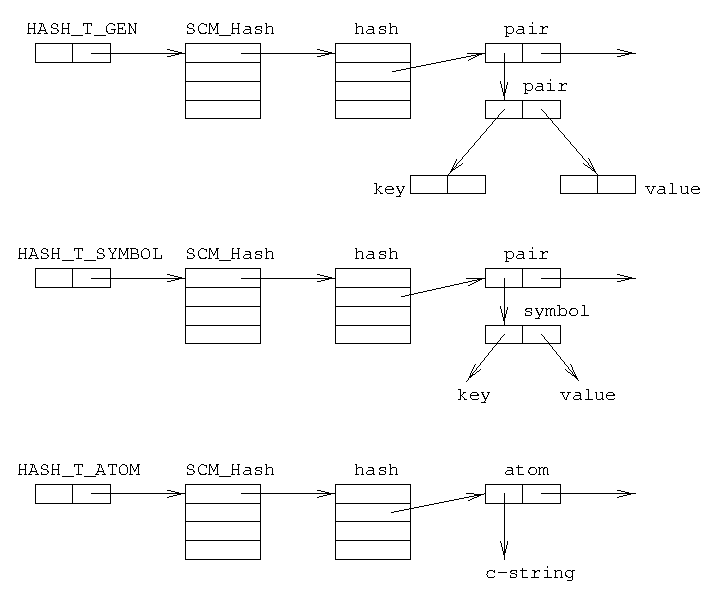
\includegraphics{hashes.eps} \par}


\caption{The various hash type}
\end{figure}


A hash is a data structure used to store key/value pairs for fast access. The
keys are assumed to be unique. The acceptable key type depends on the hash type.
For a generic type, any key may be used. For symbol hashes, only atoms or strings
are acceptable. Atom hash is very special because \emph{no value can be associated
with key}. You can use atom hash only for setting keys and testing existence
of keys.

\texttt{(make-hash} \emph{{[}type{]}}\texttt{)} --> \emph{<hash>} \\
Creates a hash. Hash types are: \texttt{SCM\_HASH\_T\_GEN} for generic (normal)
hashes, \texttt{SCM\_HASH\_T\_SYMBOL} for symbol hash and \texttt{SCM\_HASH\_T\_ATOM}
for atom hash. If no type argument is given, a generic hash is created.

\texttt{(make-symbol-hash)} --> \emph{<hash>} \\
Creates a symbol hash.

\texttt{(make-atom-hash)} --> \emph{<hash>} \\
Creates an atom hash. Atom hash has no value associated with key.

\texttt{(hash?} \emph{hash}\texttt{)} --> \emph{<boolean>} \\
Returns \texttt{\#t} if it's a hash, \texttt{\#f} otherwise. 

\texttt{(atom-hash?} \emph{hash}\texttt{)} --> \emph{<boolean>} \\
Returns \texttt{\#t} if it's an atom hash, \texttt{\#f} otherwise. 

\texttt{(symbol-hash?} \emph{hash}\texttt{)} --> \emph{<boolean>} \\
Returns \texttt{\#t} if it's a symbol hash, \texttt{\#f} otherwise. 

\texttt{(generic-hash?} \emph{hash}\texttt{)} --> \emph{<boolean>} \\
Returns \texttt{\#t} if it's a generic hash, \texttt{\#f} otherwise. 

\texttt{(hash-set!} \emph{hash key value}\texttt{)} --> \emph{<hash>} \\
Creates/changes the value associated with \emph{key.} 

\texttt{(hash-ref} \emph{hash key}\texttt{)} --> \emph{<value>} \\
Returns the value associated with the key or \texttt{\#undefined} if not found. 

\texttt{(hash-stat} \emph{hash}\texttt{)} --> \texttt{\#undefined} \\
Prints the statistics for the hash. Useful for hash optimization.

\texttt{(hash->list} \emph{hash}\texttt{)} --> \emph{<list>} \\
Returns a list containing all elements of the \emph{hash.} Elements are association
pairs where car is the key and cdr is the value. 

\texttt{(list->hash} \emph{list}\texttt{)} --> \emph{<hash>} \\
Builds a hash from an association list. 


\subsection{Number}

The documentation is again very skinny here ... refer to R5RS.

\texttt{(number?} \emph{obj}\texttt{)} --> \emph{<boolean>} \\
\texttt{(integer?} \emph{obj}\texttt{)} --> \emph{<boolean>} \\
\texttt{(real?} \emph{obj}\texttt{)} --> \emph{<boolean>} \\
\texttt{(exact?} \emph{obj}\texttt{)} --> \emph{<boolean>} \\
\texttt{(inexact?} \emph{obj}\texttt{)} --> \emph{<boolean>} \\
Type predicates. 

\texttt{(<} \emph{n1 n2 ...}\texttt{)} --> \emph{<boolean>} \emph{}\\
\texttt{(<=} \emph{n1 n2...}\texttt{)} --> \emph{<boolean>} \emph{}\\
\texttt{(>=} \emph{n1 n2 ...}\texttt{)} --> \emph{<boolean>} \\
\texttt{(>} \emph{n1 n2 ...}\texttt{)} --> \emph{<boolean>} \\
(= \emph{n1 n2 ...}\texttt{)} --> \emph{<boolean>}\\
Numeric comparisons.

\texttt{(zero?} \emph{number}\texttt{)} --> \emph{<boolean>} \texttt{}~\\
\texttt{(positive?} \emph{number}\texttt{)} --> \emph{<boolean>} \texttt{}~\\
\texttt{(negative?} \emph{number}\texttt{)} --> \emph{<boolean>} \texttt{}~\\
\texttt{(odd?} \emph{number}\texttt{)} --> \emph{<boolean>} \texttt{}~\\
\texttt{(even?} \emph{number}\texttt{)} --> \emph{<boolean>} \\
Number classes.

\texttt{(min} \emph{n1 n2 ...}\texttt{)} --> \emph{<number>} \\
\texttt{(max} \emph{n1 n2 ...}\texttt{)} --> \emph{<number>} \\
Returns the smallest, respectively the largest number of the given arguments.

\texttt{(+} \emph{n1 n2 ...}\texttt{)} --> \emph{<number>} \\
\texttt{(-} \emph{n1 n2 ...}\texttt{)} --> \emph{<number>} \\
\texttt{({*}} \emph{n1 n2 ...}\texttt{)} --> \emph{<number>} \emph{}\\
\texttt{(/} \emph{n1 n2 ...}\texttt{)} --> \emph{<number>} \emph{}\\
Arithmetic operations.

\texttt{(abs} \emph{n}\texttt{)} --> \emph{<number>} \\
Absolute value.

\texttt{(quotient} \emph{n1 n2}\texttt{)} --> \emph{<number>} \emph{}\\
\texttt{(remainder} \emph{n1 n2}\texttt{)} --> \emph{<number>} \\
\texttt{(modulo} \emph{n1 n2}\texttt{)} --> \emph{<number>} \\
Integer division and modulo operations.

\texttt{(gcd} \emph{n1 n2 ...}\texttt{)} --> \emph{<number>} \emph{}\\
\texttt{(lcm} \emph{n1 n2 ...}\texttt{)} --> \emph{<number>} \emph{}\\
Gcd and lcm of numbers.

\texttt{(floor} \emph{n}\texttt{)} --> \emph{<number>} \texttt{}~\\
\texttt{(ceil} \emph{n}\texttt{)} --> \emph{<number>} \\
\texttt{(truncate} \emph{n}\texttt{)} --> \emph{<number>} \\
\texttt{(round} \emph{n}\texttt{)} --> \emph{<number>} \\
Rounding operations.

\texttt{(exp} \emph{n}\texttt{)} --> \emph{<number>} \\
\texttt{(log} \emph{n}\texttt{)} --> \emph{<number>} \\
\texttt{(log10} \emph{n}\texttt{)} --> \emph{<number>} \\
\texttt{(sin} \emph{n}\texttt{)} --> \emph{<number>} \\
\texttt{(cos} \emph{n}\texttt{)} --> \emph{<number>} \\
\texttt{(tan} \emph{n}\texttt{)} --> \emph{<number>} \\
\texttt{(asin} \emph{n}\texttt{)} --> \emph{<number>} \\
\texttt{(acos} \emph{n}\texttt{)} --> \emph{<number>} \\
\texttt{(atan} \emph{n1 n2}\texttt{)} --> \emph{<number>} \\
\texttt{(sqrt} \emph{n}\texttt{)} --> \emph{<number>} \\
\texttt{(expt} \emph{n1 n2}\texttt{)} --> \emph{<number>} \\
Mathematical functions.

\texttt{(random)} --> \emph{<number>} \\
Generates a random number in range 0.0-1.0 exclusive. Maximum precision is 48
bits.

\texttt{(exact->inexact} \emph{n}\texttt{)} --> \emph{<number>} \\
\texttt{(inexact->exact} \emph{n}\texttt{)} --> \emph{<number>} \\
Type conversions 

\texttt{(number->string} \emph{number {[}base{]}}\texttt{)} --> \emph{<string>}
\\
\texttt{(string->number} \emph{string {[}base{]}}\texttt{)} --> \emph{<number>}\\
Convert to/from string.

\texttt{(1+} \emph{n}\texttt{)} --> \emph{<number>} \\
\texttt{(2+} \emph{n}\texttt{)} --> \emph{<number>} \\
\texttt{(1-} \emph{n}\texttt{)} --> \emph{<number>} \\
\texttt{(2-} \emph{n}\texttt{)} --> \emph{<number>} \\
 Speedy increments and decrements.

\texttt{(float-precision} \emph{digits}\texttt{)} --> \emph{old} \\
Set the number of digits after the '\texttt{.}' to display when printing a float
number.

\texttt{pi}~\\
The number PI.


\subsection{Input / output}

Input-output in Scheme is based on the concept of port. Refer to 6.6.1 in R5RS.

\texttt{(port?} \emph{obj}\texttt{)} --> \emph{<boolean>} \\
Returns \texttt{\#t} if \emph{obj} is a valid port object. 

\texttt{(input-port?} \emph{obj}\texttt{)} --> \emph{<boolean>} \\
Returns \texttt{\#t} if \emph{obj} is a valid input port object. 

\texttt{(output-port?} \emph{obj}\texttt{)} --> \emph{<boolean>} \\
Returns \texttt{\#t} if \emph{obj} is a valid output port object. 

\texttt{(current-input-port)} --> \emph{<port>}\\
\texttt{(current-output-port)} --> \emph{<port>}\\
\texttt{(current-error-port)} --> \emph{<port>} \\
Returns the current port for the default input / output / error stream. 

\texttt{(with-input-from-file} \emph{str thunk}\texttt{)} --> \emph{<anything>}\\
\texttt{(with-output-to-file} \emph{str thunk}\texttt{)} --> \emph{<anything>}
\\
Redirects standard input or output to/from the file named by \emph{str}. \emph{thunk}
is a procedure without any arguments. The value returned is the value returned
by the \emph{thunk}.

Example of redirections with \texttt{with-output-to-file} and \texttt{with-input-from-file}:

\begin{lyxcode}
>~(with-output-to-file~\char`\"{}/tmp/tst\char`\"{}~(lambda~()~(write~123)~(newline)))

\#undefined

>~(system~\char`\"{}cat~/tmp/tst\char`\"{})

123

0

>~(with-input-from-file~\char`\"{}/tmp/tst\char`\"{}~(lambda~()~(read)))

123
\end{lyxcode}
\texttt{(with-input-from-string} \emph{str thunk}\texttt{)} --> \emph{<anything>}\\
\texttt{(with-output-to-string} \emph{thunk}\texttt{)} --> \emph{<string>} \\
Redirects the standard input or output to/from \emph{string}. \emph{thunk} is
a procedure without any arguments. The value returned by \texttt{with-input-from-string}
is the value returned by the \emph{thunk}. The value returned by \texttt{with-output-to-string}
is the entire string built in \emph{thunk.}

For example:

\begin{lyxcode}
>~(with-output-to-string~(lambda~()~(write~\char`\"{}Hello~world\char`\"{})~(write~123)))

\char`\"{}\textbackslash{}\char`\"{}Hello~world\textbackslash{}\char`\"{}123\char`\"{}
\end{lyxcode}
\texttt{(open-input-file} \emph{string}\texttt{)} --> \emph{<port>} \texttt{}~\\
\texttt{(open-output-file} \emph{string}\texttt{)} --> \emph{<port>} \\
Opens the file named by \emph{string} for reading respectively writing. An error
exception is thrown if the file cannot be opened.

\texttt{(open-input-string} \emph{string}\texttt{)} --> \emph{<port>} \texttt{}~\\
\texttt{(open-output-string)} --> \emph{<port>} 

{*}{*}{*}{*} Open file for reading respectively writing. An error exception
is thrown when file cannot be opened. {*}{*}{*}{*}

\texttt{(get-output-string} \emph{<output-string-port>}\texttt{)} --> \emph{<string>}
\\
Returns the string currently built at the \emph{output-string-port}.

\texttt{(close-port} \emph{port}\texttt{)} --> \emph{<boolean>} | \emph{<string>}\\
\texttt{(close-input-port} \emph{port}\texttt{)} --> \emph{<boolean>} | \emph{<string>}\\
\texttt{(close-output-port} \emph{port}\texttt{)} --> \emph{<boolean>} | \emph{<string>}
\\
These functions close an open port. If \emph{port} is an output string port,
the string output is returned. {*}{*}{*}{*}

\texttt{(read-char {[}}\emph{port}\texttt{{]})} --> \emph{<char> | \#eof}\\
\texttt{(peek-char {[}}\emph{port}\texttt{{]})} --> \emph{<char> | \#eof} \\
Reads a character from the port passed as an argument. If no port argument is
given, the \texttt{current-input-port} is used as input port. \texttt{peek-char}
does not advance the character position of the port.

\texttt{(read-line {[}}\emph{port}\texttt{{]})} --> \emph{<string> | \#eof}\\
 Reads a line from the port passed as an argument. If no port argument is given,
the \texttt{current-input-port} is used as the input port.

\texttt{(eof-object?} \emph{obj}\texttt{)} --> \emph{<boolean>} \\
Returns \texttt{\#t} if \emph{obj} is a \texttt{\#eof.}

\texttt{(char-ready?} \emph{port}\texttt{)} --> \emph{<boolean>} \\
\textbf{Not implemented.} I'm sorry, but I don't see why you want to use this
function in a Unix environment.

\texttt{(flush-output {[}}\emph{port}\texttt{{]} )} --> \texttt{\#t}\\
Flushes the port. If no port is given, the default output port is flushed. 

\texttt{(file-position} \emph{port {[}pos{]}}\texttt{)} --> \emph{position}\\
Gets or sets the current position on a file port. If no position is given the
current position is returned. Otherwise, the current file position is set to
the \emph{pos} value.


\subsection{Error handling}

The error handling is implemented by two functions: \texttt{catch} and \texttt{throw}.
The \texttt{catch} form defines a context where errors are trapped and a function
to handle the errors occurring in that context. The \texttt{throw} function
signals an error of a specific type and provides a description of the error
in a string. The error signal is sent to the \texttt{catch} having the same
\texttt{tag} or to the innermost resp. top-level \texttt{catch} if the tag is
\texttt{\#f} resp. \texttt{\#t}. When a match is found, the handler is called
with the tag and the string thrown as arguments. When the handler terminates,
the execution resumes after the catch form and the value returned by the handler
will be returned by the catch form.

When throwing, the tag \texttt{\#t} can be used to force a top-level error with
no resume, some kind of abort.

\texttt{(catch} \emph{taglist} \emph{handler expr} \texttt{...}) \\
The \texttt{catch} construct traps exceptions occurring during the execution
of the expressions. The \emph{taglist} is a list of tags being caught. The \emph{handler}
function takes 2 arguments, a \emph{tag} and a \emph{message}. The \emph{handler}
function is called when an exception matching one of the tags has been thrown
from inside the \emph{expr}. If no exceptions occur, the catch construct returns
the value of the last expression. If an exception is trapped, the value returned
is the value returned by the handler function, if any.

\texttt{(throw} \emph{tag string}\texttt{)} \\
Sends an exception to the first catch matching the \emph{tag}. The \emph{tag}
and \emph{string} are passed to the \emph{handler} function for display purposes.
If \emph{tag} is \texttt{\#t} the top-level catch is activated. If the \emph{tag}
is \texttt{\#f} the handler of the enclosing catch is activated.

Example of a throw to an enclosing catch:

\begin{lyxcode}
>~(catch~(a~b)~(lambda~(t~m)

~~~~~~~~~~~~~~~~~(display~\char`\"{}handler:~catch:~\char`\"{})~(display~t)~

~~~~~~~~~~~~~~~~~(display~\char`\"{}~msg:~\char`\"{})~(print~m)~\#f)

~~~~~(throw~'a~\char`\"{}ERROR~A\char`\"{}))

{*}{*}{*}~throw:~tag=a~msg=ERROR~A

{*}{*}{*}~catch:~scm\_catch\_list=()

handler:~catch:~a~msg:~ERROR~A

\#f
\end{lyxcode}
Example of a \emph{throw} to first enclosing catch:

\begin{lyxcode}
>~(catch~(a~b)~(lambda~(t~m)

~~~~~~~~~~~~~~~~~(display~\char`\"{}handler:~catch:~\char`\"{})~(display~t)~

~~~~~~~~~~~~~~~~~(display~\char`\"{}~msg:~\char`\"{})~(print~m)~\#f)

~~~~~(throw~\#f~\char`\"{}ERROR~A\char`\"{}))

{*}{*}{*}~throw:~tag=\#f~msg=ERROR~A

{*}{*}{*}~catch:~scm\_catch\_list=()

handler:~catch:~\#f~msg:~ERROR~A

\#f
\end{lyxcode}
Example of a throw to top-level catch:

\begin{lyxcode}
>~(catch~(a~b)~(lambda~(t~m)

~~~~~~~~~~~~~~~~~~(display~\char`\"{}handler:~catch:~\char`\"{})~(display~t)~

~~~~~~~~~~~~~~~~~~(display~\char`\"{}~msg:~\char`\"{})~(print~m)~\#f)

~~~~(throw~\#t~\char`\"{}TOPLEVEL~ERROR\char`\"{}))

{*}{*}{*}~throw:~tag=\#t~msg=TOPLEVEL~ERROR

toplevel~restart:~k=1
\end{lyxcode}

\subsection{Module}

The module system implements private name spaces in different level. It provides
a way to control what names may be used from outside the module. This is a small
example of module definitions:

\begin{lyxcode}
(module~A

~~(export~x)

~~(define~x~10))

~

(module~B

~~(export~x)

~~(define~x~20))

~

(module~C

~~(import~A~B)

~~(print~x))

~

=>~10
\end{lyxcode}
I have a syntactic sugar notation: to access objects of a modules you can use
the module::symbol notation. Example: 

\begin{lyxcode}
(print~A::x)

=>~10
\end{lyxcode}
\textbf{Note:} the default module which holds all the Scheme definitions is
the \texttt{global} module.\\


\texttt{(module} \emph{module expr...}) \\
Creates or reuses a module. Every module uses a separate symbol hash to hold
the definitions it contains. Definitions occurring in a module will not conflict
with definitions in other modules.

\texttt{(export} \emph{symbol1 symbol2 ...}) \\
Gives a list of symbols that can be used outside of this module.

\texttt{(import} \emph{module1 module2 ...}) \\
Imports all the exported symbols of the modules listed here. The list of modules
is searched from left to right.

\texttt{(current-module)} --> \emph{module} \\
Returns the current module.

\texttt{(set-current-module} \emph{module}) \\
Sets the current module 

\texttt{(make-module} \emph{name}\texttt{)}--> \emph{module} \\
Creates a new module. If a module of that name already exists, the module associated
with name is returned.

\texttt{module-hash} --> \emph{hash} \\
Returns the hash associating names to modules.

\texttt{(module-exports} \emph{module}\texttt{)}--> \emph{list} \\
Returns the list of exported symbols. 

\texttt{(module-imports} \emph{module}\texttt{)}--> \emph{list} \\
Returns the list of imported symbols. 

\texttt{(module-symbols} \emph{module}\texttt{)}--> \emph{hash} \\
Returns a hash containing the symbol list. 

\texttt{(find-module} \emph{name}\texttt{)}--> \emph{module} \\
Searches a module in module hash and returns a module or \#f if not found. 

{*}REVIEW{*}


\subsection{Pointer}

Pointers are used to pass opaque types. You will receive pointers when you use
the \texttt{:item} keyword in the foreign function interface.

\texttt{(pointer?} \emph{obj}\texttt{)}--> \emph{<boolean>}\\
Returns \texttt{\#t} when obj is a pointer \texttt{\#f} otherwise.

\texttt{(null-pointer?} \emph{obj}\texttt{)}--> \emph{<boolean>}\\
Returns \texttt{\#t} when obj is a null pointer \texttt{\#f} otherwise.


\subsection{Process}

QScheme supports process forking and piping. The interface is described hereafter.

\texttt{(make-process} \emph{in out err string ...}\texttt{)}--> \emph{<process>}
\\
\texttt{(make-process} \emph{in out err list}\texttt{)}--> \emph{<process>}\\
\texttt{(make-process} \emph{in out err vector}\texttt{)}--> \emph{<process>}\\
Creates a new process. The values allowed for \emph{in}, \emph{out} and \emph{err}
are given in the table \ref{make_process_port_type}
\begin{table}[htb]
{\centering \begin{tabular}{|l|l|}
\hline 
Type&
Description\\
\hline 
\hline 
\texttt{:null}&
Nothing connected here\\
\hline 
\texttt{:pipe}&
Create a pipe\\
\hline 
\emph{string}&
Open a file and redirect from/to it\\
\hline 
\emph{port}&
Use an already opened port\\
\hline 
\emph{number}&
Redirect to an already opened slot\\
\hline 
\end{tabular}\par}

\caption{\label{make_process_port_type}Allowed values for make-process \emph{in out}
and \emph{err}}
\end{table}
. After this call, a new process is created and a process descriptor is returned.
If anything goes wrong, an error will be generated. 

The command specification string can be provided to \texttt{make-process} in
three different ways, namely as as in-lined strings or as a list of strings
or an array of strings . Example of such variations are given here:

\begin{lyxcode}
(make-process~:null~:pipe~:pipe~\char`\"{}ls\char`\"{}~\char`\"{}-al\char`\"{}~\char`\"{}/tmp\char`\"{})

(make-process~:null~:pipe~:pipe~'(\char`\"{}ls\char`\"{}~\char`\"{}-al\char`\"{}~\char`\"{}/tmp\char`\"{}))

(make-process~:null~:pipe~:pipe~\#(\char`\"{}ls\char`\"{}~\char`\"{}-al\char`\"{}~\char`\"{}/tmp\char`\"{}))
\end{lyxcode}
The first string argument is the full path of the command to execute and is
also the \texttt{argv{[}0{]}} of the command.

\texttt{(process?} \emph{obj}\texttt{)}--> \emph{<boolean>}\\
Returns \texttt{\#t} when obj is a process \texttt{\#f} otherwise.

\texttt{(process-pid} \emph{proc}\texttt{)}--> \emph{pid}\\
Returns the process id (pid) of the process.

\texttt{(process-input} \emph{proc}\texttt{)}--> \emph{<port}>\\
\texttt{(process-output} \emph{proc}\texttt{)}--> \emph{<port}>\\
\texttt{(process-error} \emph{proc}\texttt{)}--> \emph{<port}>\\
Returns the port corresponding to the process input, output and error stream.
You can use these ports to write or read data to/from the process.

\texttt{(process-status} \emph{proc}) --> \emph{status}\\
Returns the status of a process.

\texttt{(process-wait} \emph{proc}\texttt{)}--> \emph{status}\\
Waits for a process to terminate. If \emph{proc} is \texttt{\#t}, waits for
any process to terminate. Returns the exit status of the process. After a \texttt{process-wait}
completes\emph{,} the process does not exist anymore and the ports are closed.
You could also access the status of the process with the \texttt{process-status}
function.

\texttt{(process-use-execv} \emph{flag}\texttt{)}--> \emph{oldvalue}\\
Determines if processes are created with \texttt{execv} or \texttt{execvp}.
When execv is used, first argument must be the full path to the command. When
\texttt{execvp} is used, the \texttt{PATH} environment variable is search to
find the command. Returns the value of the flag before the call. 

\begin{description}
\item [Note:]By default, \texttt{execvp} is used.
\end{description}

\subsection{Threads}

\texttt{(thread} \emph{thunk}\texttt{)}--> \emph{thread}\\
Invoke \emph{thunk} with no arguments in a new thread. Returns \emph{thread},
a thread descriptor. When execution of \emph{thunk} returns, the thread created
to invoque \emph{thunk} terminates.

\texttt{(thread?} \emph{obj}\texttt{)}--> \emph{boolean}\\
Returns \texttt{\#t} if \emph{obj} is a thread descriptor, \texttt{\#f} otherwise.

\texttt{(thread-id} \emph{thread}\texttt{)}--> \emph{number}\\
 Returns the \emph{pthread id} associated with \emph{thread.}

\texttt{(current-thread)}--> \emph{thread}\\
Returns the \emph{thread} descriptor for current thread.

\texttt{(thread-running?} \emph{thread}\texttt{)}--> \emph{boolean}\\
Returns \texttt{\#t} if thread is currently running, \texttt{\#f} otherwise.

\texttt{(thread-wait} \emph{thread}\texttt{)}--> \texttt{\#undefined}\\
Wait until \emph{thread} terminates. 

\texttt{(thread-kill} \emph{thread}\texttt{)}--> \texttt{\#undefined}\\
Terminate \emph{thread.}

\texttt{(thread-exit} \emph{thread}\texttt{)}--> \texttt{\#undefined}\\
Terminates current \emph{thread}. This function never returns.

\texttt{(thread-dump} \emph{thread}\texttt{)} --> \texttt{\#undefined} \\
Dump the content of a thread. Mostly for debugging purpose.


\subsection{Mutexes}

A mutex is a MUTual EXclusion device, and is useful for protecting shared data
structures from concurrent modifications, and implementing critical sections
and monitors.

A mutex has two possible states: \emph{unlocked} and \emph{locked}. A mutex
can never be owned by two different threads simultaneously. A thread attempting
to lock a mutex that is already locked by another thread is suspended until
the owning thread unlocks the mutex first.

\texttt{(make-mutex)} --> \emph{mutex}\\
Create a new \emph{mutex}

\texttt{(mutex?} \emph{obj}\texttt{)} --> \emph{boolean} \\
Returns \texttt{\#t} if obj is a \emph{mutex}, \texttt{\#f} otherwise

\texttt{(mutex-lock} mutex\texttt{)} --> \texttt{\#undefined}\\
Lock \emph{mutex}. If \emph{mutex} is already locked, thread execution is suspended
until \emph{mutex} is unlocked

\texttt{(mutex-try-lock} \emph{mutex}\texttt{)} --> \emph{boolean}\\
Try to lock \emph{mutex}. If \emph{mutex} is already locked, \texttt{\#f} is
returned immediately, otherwise the \emph{mutex} is locked and \texttt{\#t}
is returned.

\texttt{(mutex-unlock} \emph{mutex}\texttt{)} --> \texttt{\#undefined}\\
Unlock \emph{mutex}


\subsection{Semaphores}

Semaphores are counters for resources shared between threads. The basic operations
on semaphores are: increment the counter atomically, and wait until the counter
is non-null and decrement it atomically.

\texttt{(make-semaphore} \emph{{[}value{]}}) --> \emph{semaphore}\\
Create a new \emph{semaphore} object.

\texttt{(semaphore?} \emph{object}\texttt{)} --> \emph{boolean} \\
Returns \texttt{\#t} if \emph{object} is a semaphore, \texttt{\#f} otherwise.

\texttt{(semaphore-wait} \emph{semaphore}\texttt{)} --> \texttt{\#undefined}

Suspend the calling thread until \emph{semaphore} has non-zero count, then decrease
the semaphore count.

\texttt{(semaphore-try-wait} \emph{semaphore}\texttt{)} --> \emph{boolean} \\
Non blocking variant of \texttt{semaphore-wait}. If \emph{semaphore} has non-zero
count, the count is atomically decreased and \texttt{\#t} is returned. If \emph{semaphore}
count is zero, \texttt{\#f} is returned.

\texttt{(semaphore-post} \emph{semaphore}\texttt{)} --> \texttt{\#undefined}
\\
Atomically increases the count of \emph{semaphore}.

\texttt{(semaphore-get-value} \emph{semaphore}\texttt{)} --> \emph{number} \\
Return the count assiociated to the \emph{semaphore}.


\subsection{Miscellaneous}

\texttt{(apropos} \emph{string}\texttt{)}--> \emph{list}\\
Returns a list of known symbols that contains the \emph{string.}

\texttt{(whatis} \emph{string}\texttt{)}--> \texttt{\#undefined}\\
Searches the \texttt{whatis.qs} file and displays the definitions of the words
matching \emph{string}. The \texttt{whatis.qs} file is built with the \texttt{mkwhatis}
script. The string \emph{string} may end with a wild card character (\#\textbackslash{}\textasciitilde{}),
in which case all entries beginning with the significant part of \emph{string}
will be returned.

Example of \texttt{whatis} usage :

\begin{lyxcode}
>~(whatis~\char`\"{}set\textasciitilde{}\char`\"{})~

(set!~VAR~EXPR)~=>~VALUE~~~~~~~~~~~~~~~~~~~{[}SYNTAX{]}~

~~Evaluates~EXPR~and~stores~the~resulting~value~in~

~~the~location~to~which~VAR~is~bound.

(set-car!~PAIR~OBJ)~=>~\#undefined~~~~~~~~~~~{[}~R5RS{]}~

~~Stores~OBJ~in~the~car~field~of~PAIR.

(set-cdr!~PAIR~OBJ)~=>~\#undefined~~~~~~~~~~~~{[}R5RS{]}~~\\
~~Stores~OBJ~in~the~cdr~field~of~PAIR.

(set-current-module~MODULE)~=>~MODULE~~~~~{[}QScheme{]}~

~~Set~MODULE~as~current~module~for~symbol~search.

(set-aux!~OBJ~VAL)~=>~NULL~~~~~~~~~~~~~~~~{[}QScheme{]}~

~~Associate~a~value~to~the~aux~pointer~of~object.~

~~THIS~IS~A~DANGEROUS~FUNCTION.
\end{lyxcode}

\section{Foreign function interface}

QScheme provides a way to dynamically load dynamic libraries, to call functions
of that library and to share variables with libraries.


\subsection{Loading a dynamic library \label{Qscm_loadlib}}

\texttt{(load-library} \emph{name}\texttt{)}--> \emph{<boolean>} \\
Attempts to load la dynamic library. If the dynamic linkage succeeds and the
library contains a function named \texttt{scm\_init\_}\emph{name} QScheme will
call this function to initialize the module. (See \texttt{scm\_init\_regex}
in \texttt{regex.c} for an example.)


\subsection{Calling a foreign function}

To call a foreign function, you have to declare it first. As an example, here
is the declaration of the \texttt{system} and \texttt{printf} functions from
\texttt{libc}:

\begin{lyxcode}
(define~system~(make-extfunc~{*}lib{*}~:int~\char`\"{}system\char`\"{}~'(:string)))

(define~printf~(make-extfunc~{*}lib{*}~:void~\char`\"{}printf\char`\"{}~'(:string~.~:any)))
\end{lyxcode}
After that, you can use \texttt{system} and \texttt{printf} just as is they
were part of QScheme:

\begin{lyxcode}
>~(printf~\char`\"{}May~I~?~\%d~\%s\textbackslash{}nIt~works...\textbackslash{}n\char`\"{}~10~\char`\"{}hello~world\char`\"{})~

May~I~?~10~hello~world~It~works...

>
\end{lyxcode}
\texttt{(make-extfunc} \emph{libname ret-type ext-name arglist}\texttt{)}-->
\emph{<extfunc>} \\
Creates a new Scheme object which can be used to call the foreign function \emph{ext-name}

You can pass strings as arguments to a foreign function. The string is passed
to the function as is. If the size of the string should be adjusted, this may
be done with the \emph{string-} functions. For instance, this QScheme function
lists the contents of a file using the \emph{stdio} functions:

\begin{lyxcode}
(define~(type~file)

~~(let~((fd)~(buf)~(bufsize~256))

~~~~(set!~fd~(fopen~file~\char`\"{}r\char`\"{}))

~~~~(if~(not~(null-pointer?~fd))

~~~~~~~~(begin

~~~~~~~~~~(while~

~~~~~~~~~~~(not~(null?~

~~~~~~~~~~~~~~~~~(fgets

~~~~~~~~~~~~~~~~~~(set!~buf~(make-string~bufsize~\#\textbackslash{}space))

~~~~~~~~~~~~~~~~~~bufsize

~~~~~~~~~~~~~~~~~~fd)))

~~~~~~~~~~~(printf~\char`\"{}\%s\textbackslash{}n\char`\"{}~(string-chop~buf)))

~~~~~~~~~~(fclose~fd))

~~~~~~~~(printf~\char`\"{}cannot~open~file~\%s\char`\"{}~file))))
\end{lyxcode}
Note how we pass the \texttt{buf} to the \texttt{fgets} function and how we
use it afterwards. 


\subsection{Using a foreign variable}

QScheme can also access variables defined in dynamic libraries. (see \texttt{load-library}:
\ref{Qscm_loadlib}). 

\texttt{(make-extern-variable} \emph{libname type name}\texttt{)}--> \emph{<external-variable>}
\\
Creates an external variable. \emph{libname} is a string containing the path
to the dynamically loaded library. The library will be loaded on demand. The
\emph{type} is a keyword as described in the table 
\begin{table}[htb]
\vspace{0.3cm}
{\centering \begin{tabular}{|l|l|l|}
\hline 
Type&
C type&
Description\\
\hline 
\hline 
\texttt{:char}&
\texttt{char} &
a character\\
\hline 
\texttt{:short}&
\texttt{short}&
a short integer\\
\hline 
\texttt{:long}&
\texttt{long}&
a long integer\\
\hline 
\texttt{:float}&
\texttt{float}&
a float number\\
\hline 
\texttt{:double}&
\texttt{double}&
a double float number\\
\hline 
\texttt{:string}&
\texttt{char {*}}&
a \texttt{malloc}-ed string.\\
\hline 
\texttt{:string-buffer}&
\texttt{char {*}}&
a pointer to a char buffer\\
\hline 
\texttt{:scheme}&
\texttt{SOBJ}&
a pointer to a Scheme object\\
\hline 
&
&
\\
\hline 
\end{tabular}\par}\vspace{0.3cm}


\caption{\label{extvar_type}Type of external variables}
\end{table}
\ref{extvar_type}. The \emph{name} is a string containing the name of the variable
as defined in the module. 

The type of external strings is specified according to the string allocation
scheme. We have to deal with the following cases: 

\begin{itemize}
\item the string is stored in a static array of characters.
\item the string is dynamically allocated with \texttt{malloc}. 
\end{itemize}
When referring to a dynamically allocated string, you have to use the \texttt{:string}
type. Changing such a string from QScheme will first free the memory then \emph{malloc}
a fresh copy of the string.

When referring to a string stored in a static character buffer, you must use
the \texttt{:string-buffer} type. In this case the value is just copied in the
buffer. Beware that no range check occurs. From QScheme, don't try to assign
a string bigger than the static buffer size. 

Look at \texttt{tstlib.c} and \texttt{tstlib.defs} for an example that uses
static and dynamic strings in a dynamic library.


\subsection{A trivial example}

Here is an example of how to share variable values between C and QScheme. In
your C code, you have the following:

\begin{lyxcode}
int~shared\_var;

~

void~test\_func()~\{

~~printf(\char`\"{}shared\_var~=~\%d\textbackslash{}n\char`\"{},~testvar\_w);

\}
\end{lyxcode}
To access the variable \texttt{shared\_var} and the function \texttt{test\_func}
from Qscheme, you may use the following definitions:

\begin{lyxcode}
(define~{*}lib{*}~\char`\"{}./tstlib.so\char`\"{})

(define~shared-var~(make-extern-variable~{*}lib{*}~:int~\char`\"{}shared\_var\char`\"{})

(define~test-func~(make-extfunc~{*}lib{*}~:void~\char`\"{}test\_func\char`\"{}~'())
\end{lyxcode}
Then you can get and set values like this:

\begin{lyxcode}
>~(set!~shared-var~100)

>~(test-func)

shared\_var~=~100

>~(display~shared-var)~(newline)

100

>
\end{lyxcode}
\begin{description}
\item [Warning:]You must use \texttt{define} to bind a symbol to an external variable
and \texttt{set!} to modify directly the value of the variable.
\end{description}

\subsection{Declaring and using foreign types}

QScheme can create new Scheme object types at run-time. 

\texttt{(make-type} \emph{name}\texttt{)}--> \emph{<type-number>} \\
Creates a new type of Scheme object. The number returned is the internal type
number.

\texttt{(define-type} \emph{<keyword> | <string> | <symbol>}\texttt{)}--> \texttt{\#undefined}\\
Creates a new type of Scheme object. This is just a wrapper around the \texttt{make-type}
function.

\texttt{(internal-type-list)} --> \emph{<list>}\\
Returns a list of strings representing the know types.

\texttt{(get-aux} \emph{obj}\texttt{)}--> \emph{<obj>} \texttt{}~\\
\texttt{(set-aux!} \emph{obj value}\texttt{)}--> \texttt{\#undefined }~\\
\texttt{(clear-aux!} \emph{obj}\texttt{)}--> \texttt{\#undefined} \\
\texttt{(null-aux?} \emph{obj}\texttt{)}--> \emph{<boolean>}\\
These functions test and change the \emph{aux} field of an object. The \emph{aux}
field is large enough to store a pointer.

\begin{description}
\item [Warning:]the \texttt{set-aux!} and \texttt{clear-aux!} do \textbf{not} check
the type of object. You may alter whatever Scheme object you want, and this
may lead to regrettably unpredictable results. You should not modify the \emph{aux}
field of ordinary Scheme objects, because this field may be used for specific
purpose. (for example, the \emph{aux} field of a pair is the \emph{car} field).
\end{description}
\texttt{(add-type-finalizer} \emph{type proc}\texttt{)}--> \texttt{\#undefined}
\emph{}\\
Defines a procedure to be executed when an object of this \emph{type} is released
by the garbage collector. When called the \emph{proc} is a given the object
to be destroyed as argument.

\begin{description}
\item [Note:]the \emph{proc} is a procedure which is executed in the top-level context,
which means the procedure \emph{should not use any local references!} 
\end{description}
A new type maybe used in conjunction with the \texttt{make-extfunc} procedure.
For example:

\begin{lyxcode}
(define-type~:file)

~

(define~fopen

~~(make-extfunc~\char`\"{}\char`\"{}~:file~\char`\"{}fopen\char`\"{}~'(:string~:string)))

~

(define~fprintf

~~(make-extfunc~\char`\"{}\char`\"{}~:void~\char`\"{}fprintf\char`\"{}~'(:file~:string~.~:any)))

~

(define~\_fclose~(make-extfunc~\char`\"{}\char`\"{}~:void~\char`\"{}fclose\char`\"{}~'(:file)))

~

(define~(fclose~x)

~~(if~(not~(null-aux?~x))~(\_fclose~x))

~~(clear-aux!~x))

~

(add-type-finalizer~

~\char`\"{}file\char`\"{}

~(lambda~(x)~(fclose~x)))
\end{lyxcode}
In this example, the \emph{finalizer} procedure closes the file. This guarantees
that the file will not stay open when the Scheme objects that were using it
have all vanished.


\section{Running QScheme}


\subsection{Syntax}

\begin{lyxcode}
qscheme~{[}options{]}~{[}file{]}~{[}-{}-{]}~{[}argument~...{]}
\end{lyxcode}

\subsection{Options}

\begin{description}
\item [\texttt{-hs=}\emph{N}~\texttt{-{}-heap-size=}\emph{N}]the heap block size.
The number of objects that can be stored in a heap block is \emph{N}{*}1024,
and the number of block heaps we can use is only limited by the virtual memory
of the computer.
\item [\texttt{-ds=}\emph{N}~\texttt{-{}-stack-size=}\emph{N}]the stack size. The
number of object references that can be stored on the stack. \emph{N} is a number
of kilobytes.
\item [\texttt{-ni}~\texttt{-{}-no-init}]do not read the initial file.
\item [\texttt{-i}~\texttt{-{}-interractive}]Force interactive mode. If \texttt{file}
are specified, they are loaded first.
\item [Note:]The heap block size does not seem to have big impact on then performance
yet. The default value is 32k now which seems to be a good value.
\end{description}

\subsection{Environment}

During the initialization of QScheme, the interpreter tries to load a file named
\texttt{s.scm.} The initialization file will be looked for in the following
directories:

\begin{itemize}
\item in the current directory
\item in the directories designated by the \texttt{QS\_LIB} environment variable.
You can specify as many directories as you want by just delimiting them with
the '\texttt{:}' character. For example:
\end{itemize}
\begin{lyxcode}
QS\_LIB=/usr/local/share/qscheme:\$HOME/qscheme

export~QS\_LIB
\end{lyxcode}
The search order is as indicated above.


\subsection{Scripting}

You can also use QScheme in a standard Unix script context. For example

\begin{lyxcode}
\#!/usr/local/bin/qscheme~-ni~-ds=128

(display~\char`\"{}Hello~world\char`\"{})

(newline)
\end{lyxcode}
will produce the expected outpout:

\begin{lyxcode}
Hello~world
\end{lyxcode}
Easy, isn't it...


\section{Data types {*}REVIEW{*}}


\subsection{Built-in data types}

The table \ref{type_table}
\begin{table}[htb]
\vspace{0.3cm}
{\centering \begin{tabular}{|l|l|l|}
\hline 
Type&
Description&
Example\\
\hline 
\hline 
SOBJ\_T\_VOID&
when returned by eval no print occurs&
\\
\hline 
SOBJ\_T\_PAIR&
result of a cons&
(cons 1 2) => (1 . 2)\\
\hline 
SOBJ\_T\_INUM&
small integer number. 31 bits&
123\\
\hline 
SOBJ\_T\_FNUM&
double&
1.2\\
\hline 
SOBJ\_T\_BNUM&
big integer number&
108230980172834891\\
\hline 
SOBJ\_T\_ATOM&
an atom&
'a\\
\hline 
SOBJ\_T\_KEYWORD&
starts with ':' and evaluates to itself&
:keyword\\
\hline 
SOBJ\_T\_SYMBOL&
a symbol&
symbol\\
\hline 
SOBJ\_T\_LSYMBOL&
local symbol&
x\\
\hline 
SOBJ\_T\_LABEL&
label for named let&
\\
\hline 
SOBJ\_T\_MODULE&
module description&
\\
\hline 
SOBJ\_T\_CHAR&
a character&
\#\textbackslash{}space\\
\hline 
SOBJ\_T\_STRING&
a string&
``Hello world''\\
\hline 
SOBJ\_T\_PRIM&
internal VM primitive&
\%push\\
\hline 
SOBJ\_T\_CPRIM&
primitive coded in C&
display\\
\hline 
SOBJ\_T\_SYNTAX&
syntax object&
define\\
\hline 
SOBJ\_T\_CODE&
code without parameter&
\\
\hline 
SOBJ\_T\_PROC&
procedure: has parameter(s)&
\\
\hline 
SOBJ\_T\_ENV&
environment&
\\
\hline 
SOBJ\_T\_CLOSURE&
closure&
\\
\hline 
SOBJ\_T\_MACRO&
macro&
\\
\hline 
SOBJ\_T\_PORT&
port&
\\
\hline 
SOBJ\_T\_BOOLEAN&
\#t or \#f&
\\
\hline 
SOBJ\_T\_UNBOUND&
value of an unbound symbol&
\\
\hline 
SOBJ\_T\_UNDEFINED&
value of an undefined value&
\\
\hline 
SOBJ\_T\_EOF&
the EOF value&
\\
\hline 
SOBJ\_T\_CONT&
continuation&
\\
\hline 
SOBJ\_T\_ARRAY&
array&
\\
\hline 
SOBJ\_T\_HASH&
hash&
\\
\hline 
SOBJ\_T\_POINTER&
generic pointer&
\\
\hline 
SOBJ\_T\_EXTFUNC&
external function, dynamically loaded&
\\
\hline 
SOBJ\_T\_EXTVAR&
reference to an external variable&
\\
\hline 
SOBJ\_T\_VAR&
reference to an external variable&
\\
\hline 
SOBJ\_T\_VMFUNC&
VM extension functions&
\\
\hline 
SOBJ\_T\_CCNTXT&
catch context&
\\
\hline 
SOBJ\_T\_USER&
user-defined types&
\\
\hline 
\end{tabular}\par}\vspace{0.3cm}


\caption{\label{type_table}Builtin Scheme object type}
\end{table}
 describes the currently defined Scheme object types.


\subsection{Adding new Scheme object types from C}

The built-in data types can be extended by user defined data types. New user
types can be registered using the following structures and API.

\texttt{SOBJ\_TYPE\_DESCR} 

\begin{LyXParagraphIndent}{0.4cm}
This is the structure describing a type. See the definitions in file \texttt{s.h} 

\end{LyXParagraphIndent}

\texttt{SOBJ\_TYPE\_DESCR scm\_type\_hook{[}SOBJ\_T\_MAX{]}}

\begin{LyXParagraphIndent}{0.4cm}
This is the global type structure\@. You don't have to manipulate directly
this table. 

\end{LyXParagraphIndent}

\texttt{int scm\_add\_type(SOBJ\_TYPE\_DESCR {*}type)}

\begin{LyXParagraphIndent}{0.4cm}
This function adds a new type to the \texttt{scm\_type\_hook{[}{]}} array. The
integer returned is the type descriptor.

\end{LyXParagraphIndent}

To add a new Scheme object type, you have to go through the following steps:

\begin{itemize}
\item Write code to mark and sweep this new type of object
\item Write code to display this new type of object 
\item Fill out a \texttt{SOBJ\_TYPE\_DESCR} structure with the functions you just
wrote
\item call \texttt{scm\_add\_type} and remember the value returned. This is your new
type descriptor.
\item That's all.
\end{itemize}
A real and non-trivial working example of how to build a new Scheme object type
can be found in the \texttt{regex.c} file. 

\begin{description}
\item [Note:]The \texttt{dyntype.c} file can be use as prototype to build a new type
from the C language. Just copy it and rename the ``xxx'' string with the name
of your new type.
\end{description}

\section{Internal representation of QScheme objects}

Every QScheme object is either a pointer to a cell or an immediate small integer. 


\subsection{QScheme cells}

All non immediate QScheme objects are stored in a heap, which is simply an array
of \texttt{Sobject}

structure. A \texttt{Sobject} structure contains the following fields:

\begin{itemize}
\item a type field, describing the type of Scheme object.
\item enough bytes to store 2 pointers.
\end{itemize}
QScheme expects that following assumptions are strictly verified:

\begin{enumerate}
\item The size of the Sobject structure must be a multiple of 2. 
\item The heap starts on an address which is a multiple of 2.
\end{enumerate}
Because of this, the pointers to Scheme object are always even, which means
that bit 0 is always 0. 

If a type needs more data than the 2 pointers space provided by a cell, it has
to allocate more space in the system heap by using the \texttt{scm\_must\_alloc}
and \texttt{scm\_free} functions.


\subsection{Immediate small integers}

Immediate small integers have bit 0 set to 1. The other bits of the word contain
the true integer value. So on a machine where pointer are on 32 bits, the immediate
number are coded on 31 bits.


\subsection{Other Objects}


\subsubsection{Procedures}

A procedure is implemented as follow:

\begin{lyxcode}
<proc>~~~~~=~{[}~<envFrame>~|~<code>~{]}

<envFrame>~=~<next>~<nslots>~<bindings>

<code>~~~~~=~<envList>~<size>~<nargs>~<optargs>~<code-slot>~...
\end{lyxcode}
The \texttt{envFrame} pointer points to an Environment Frame which is cloned
at runtime to contain the current bindings.

The \texttt{envList} is a pointer to the symbolic representation of the environment
as built at compilation time. The compile-time environment is a list of \texttt{localvar}
symbols. 

\begin{lyxcode}
<localvar>~=~{[}~<symbol>~|~<depth>~<ofs>~{]}
\end{lyxcode}

\subsubsection{Numbers}

{*}REVIEW{*} 

{*}{*}{*} Yes, numbers ... {*}{*}{*}


\section{Virtual Machine}


\subsection{Introduction}

The virtual machine consists of a set of registers and a stack. See table \ref{vm_registers}
\begin{table}[htb]
{\centering \begin{tabular}{|l|l|}
\hline 
Register&
Description\\
\hline 
\hline 
ip&
the instruction pointer\\
\hline 
sp&
the stack pointer\\
\hline 
TOS&
the top of stack register. You can consider TOS as a cache.\\
\hline 
cont&
the pointer to the current continuation frame.\\
\hline 
env&
the pointer to the current dynamic environment\\
\hline 
\end{tabular}\par}

\caption{\label{vm_registers}Virtual Machine registers}
\end{table}


The stack is used both at compile-time and at run-time. 

At compilation time, QScheme uses the stack as temporary workspace to generate
code. This is done to limit the number of cells created and as consequence the
number of GCs (garbage collections).

At run time, QScheme uses the stack to store function arguments, runtime environment,
catches and partial continuations\@.

The default stack size is 32000 pointers.. This default can be changed on the
command line. 

Presently, stack overflow and underflow conditions are not caught during execution,
to avoid the related execution overhead and raise the performance of the VM
- speed matters.

The virtual machine is in the file \texttt{vm2.c} file.


\subsection{Internal opcodes}

The internal opcodes are stored in the table \texttt{symbols} local to the function
\texttt{scm\_vm()} in the file \texttt{vm2.c} .

A pointer to this table is provided during initialization of the virtual machine. 


\subsection{Various things to know}

Things to know

\begin{itemize}
\item during the sweep phase, all accessible cells have the gc mark bit set. Because
I don't want to mask to obtain the true type, you will have to cope with the
fact that the primitive testing the type will be fooled. (the \texttt{scm\_display}
function is anyway GC-proof (for debugging))
\item the nargs field in the code header is the number of arguments expected \emph{including}
the optional argument. This means that nargs is the number of argument slots
a function will receive.
\end{itemize}

\section{QScheme libraries}


\subsection{Perl regular expressions - regex.so}

The Perl regular expression module is a really good example of an extension
module (a module that you can load while QScheme is running). This is an interesting
example, because it dynamically adds a new syntactic token. 

All the functions of this library will be added in the module \texttt{regex.}

The new syntaxic token \texttt{\#/}\emph{regex}\texttt{/}\emph{opts} compiles
a new regular expression. The options are:

\vspace{0.3cm}
{\centering \begin{tabular}{|c|l|}
\hline 
Options&
Description\\
\hline 
\hline 
a&
anchored. Just like if re was enclosed between \textasciicircum{} and \texttt{\$}\\
\hline 
i&
ignore case\\
\hline 
s&
. matches also newlines\\
\hline 
m&
multi-line\\
\hline 
x&
extended\\
\hline 
U&
ungreedy\\
\hline 
X&
extra\\
\hline 
\end{tabular}\par}
\vspace{0.3cm}

Look at the \texttt{pcre} manual page for more informations.

The following functions deal with regular expressions:

\texttt{(regex::isa?} \emph{obj}\texttt{)} --> \emph{<boolean>}

\begin{LyXParagraphIndent}{0.4cm}
Returns true when \emph{obj} is a compiled regular expression.

\end{LyXParagraphIndent}

\texttt{(regex::match} \emph{re string}\texttt{)} --> \emph{<number> | \#f}

\begin{LyXParagraphIndent}{0.4cm}
Returns the number of match found or \#f if no match occurred.

\end{LyXParagraphIndent}

\texttt{(regex::sub} \emph{n}\texttt{)} --> \emph{<string>} \texttt{| \#f}

\begin{LyXParagraphIndent}{0.4cm}
Returns the value of last nth sub-match.

\end{LyXParagraphIndent}

\texttt{(regex::\$}\emph{n}\texttt{)} --> \emph{<string>} \texttt{| \#f}

\begin{LyXParagraphIndent}{0.4cm}
Equivalent to \texttt{(regex::sub} \emph{n}\texttt{)}, where n is a number from
0 to 9. 

\end{LyXParagraphIndent}

\end{document}
